\documentclass[a4paper, 11pt]{article}
\usepackage{geometry}
\geometry{letterpaper, margin=1in}
\usepackage{amsmath}
\usepackage{amssymb}  
\usepackage{amsthm}
\usepackage{ulem} 
\usepackage{graphicx}
\usepackage{cancel} 
\usepackage{enumitem} 
\graphicspath{ {images/} }


\newtheorem*{theorem}{Theorem}
\newtheorem*{corollary}{Corollary}
\newtheorem*{lemma}{Lemma}
\newtheorem*{definition}{Definition}

\begin{document}
	%Header-Make sure you update this information!!!!
	\noindent
	\large\textbf{Thermal Physics - PH441} \hfill \textbf{John Waczak} \\
	\normalsize Day 20 \hfill  Date: \today \\
	
	
\subsection*{More On Density Of States}	
	\par\noindent\rule{\textwidth}{0.4pt};	
	Let's derive the Fermi-energy. Last time we had
		\begin{equation*}
			N = \frac{V}{2\pi^2}\Big(\frac{2m}{\hbar^2}\Big)^{3/2}\frac{2}{3}\varepsilon_f^{3/2}
		\end{equation*}
	Using this we can solve for the Fermi energy to find: 
		\begin{equation*}
			\varepsilon_f = \frac{\hbar^2}{2m}\Big(\frac{N2\pi^2}{V}\Big)^{2/3}
		\end{equation*}
	and so we can simplify our density of states to arrive at
		\begin{equation*}
			D(\varepsilon) = \frac{3}{2}N\frac{\varepsilon^{1/2}}{\varepsilon_f^{3/2}}
		\end{equation*}	
	
	\noindent Now we can use $\varepsilon_f$ to define a whole bunch of \textit{Fermi} things. 
		\begin{align*}
			k_f &= \Big(\frac{N}{V}2\pi^2\Big)^{1/3} \\ 
			p_f &= \hbar k_f \\ 
			v_f &= \frac{p_f}{m} \\ 
			T_f &= \frac{\varepsilon_f}{k_B}
		\end{align*}
		

\subsection*{Example}
	\par\noindent\rule{\textwidth}{0.4pt};	
	Solve for U of a Fermi-gas at zero-Temperature: 
		\begin{align*}
			U &= \int_0^\infty D(\varepsilon)\varepsilon f(\epsilon)d\varepsilon
		\end{align*}
	Where $D(\varepsilon)$ tells us how many orbitals there are at an energy $\varepsilon$ per unit energy and $f(\varepsilon)$ is the Fermi-Dirac distribution function that tells us what fraction of orbitals are occupied at a given $\varepsilon$. At zero temperature $f(\varepsilon)$ becomes a step function that turns off at $\varepsilon_f$. Thus we have 
		\begin{align*}
			U_{T = 0} &= \int_0^{\varepsilon_f} D(\varepsilon)\varepsilon d\varepsilon \\
			&= \frac{3}{2}N\int_0^{\varepsilon_f} \frac{\varepsilon^{3/2}}{\varepsilon_f^{3/2}}d\varepsilon \\ 
			&= \frac{3}{5}\varepsilon_f
		\end{align*}
		
\subsection*{Example} 
	\par\noindent\rule{\textwidth}{0.4pt};
	How would you find $C_v$? 
		\begin{align*}
			C_v &= \Big(\frac{\partial U}{\partial T}\Big)_{V,N} \\ 
			U &= \int_0^\infty D(\varepsilon)f(\varepsilon)\varepsilon d\varepsilon \\ 
		\end{align*}
	\begin{figure}[!hbt]
		\centering
		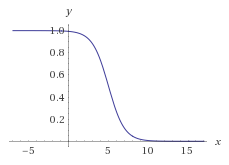
\includegraphics[scale = 1.0]{fermiDirac}
		\caption{The shape of the Fermi-Dirac distribution}
	\end{figure}
\end{document}

























